\section{El panel de acciones}
\label{s5:sec:panel_dcha}
Como se ha descrito anteriormente, cada c�mara que forma el juego
posee sus propios scripts que sirven para crear e interactuar con los
elementos que ah� aparecen. En esta secci�n se describen los
componentes que forman la parte derecha de la pantalla, esto es, la
relacionada con las acciones que puede realizar el robot, y como estas
se pueden combinar en forma de paneles.

\subsection{Bot�n de comando: Prefab y script asociado}
Para crear los botones en los que el usuario puede hacer click y
seleccionar una acci�n se ha decidido utilizar \emph{sprites} con la
imagen que se desea mostrar. As� mismo, como se desea que el color de
fondo cambie, en vez de utilizar sprites con colores diferentes, se ha
decidido utilizar sprites transparentes, y utilizar un cubo de fondo
que cambi�ndole el material da la sensaci�n de que el fondo del sprite
se ha cambiado. En la figure~\ref{s5:fig:action_prefab} se puede ver
un esquema de como est� realizado.

\begin{figure}
  \centering
  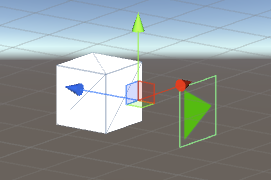
\includegraphics[width=0.3\textwidth]{images/action_prefab.png}
  \caption{Botones de acci�n formados por un cubo y un sprite con el
    fondo transparente.}
  \label{s5:fig:sction_prefab}
\end{figure}

Para poder interactuar con el bot�n, el sprite tiene asociado un
componente de colisi�n en 2D, permitiendo detectar cuando es
pulsado. Para cambiar el color del fondo, basta con buscar el �nico
\emph{MeshRenderer} del prefab (el �nico que existe es el asociado al
cubo).


Asociado al sprite del prefab, se encuentra el siguiente script
(\texttt{Action.cs}), que posee una definici�n de todos los tipos de
acciones, as� de las acciones a realizar cuando el bot�n es pulsado:

\begin{lstlisting}[caption={Action.cs Script encargado de reaccionar
      frente a las pulsaciones de los botones}]
using UnityEngine;
using System.Collections;

/**
 * Posibles tipos de comandos
 */
public enum ActionType{
	up,
	right,
	left,
	jump,
	play,
	light,
	trash,
	pause,
	p1,
	p2,
	none
}

/**
 * Listener de las pulsadciones de los botones. Segun el comando a ejecutar
 * invoca a un metodo u otro 
 */
public class Action : MonoBehaviour {
  //Tipo de accion que representa el boton
  public ActionType actionType;
  
  
  
  public void OnMouseUpAsButton()
  {
    switch (this.actionType) {
      case ActionType.play:
        Director.S.play();
        break;
      case ActionType.trash:
        Director.S.trash();
	break;
      case ActionType.none: //si pulsamos en una accion vacia, es que estamos en el panel
        Panel p = transform.parent.transform.parent.GetComponent<Panel>(); 
	p.activatePanel();
	break;
      default: //acciones para el robot
      Director.S.addAction (this.actionType);
      break;
    }
  }
}
\end{lstlisting}


\subsection{Layout}
\label{s5:subsec:layout}
Para la creaci�n de la interfaz derecha de la pantalla, partimos de la
configuraci�n inicial de la pantalla mostrada en la
figura~\ref{s5:fig:interfaz_white} (es decir, los
siguientes prefabs ya se encuentran instanciados en la escena, no a
trav�s del c�digo):

\begin{figure}[h]
  \centering
  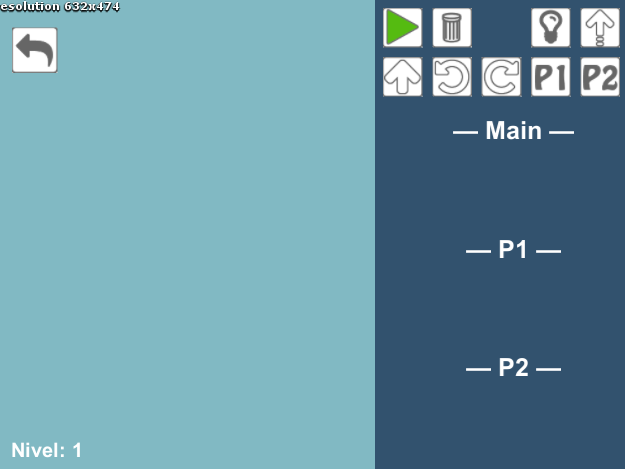
\includegraphics[width=0.6\textwidth]{images/interfaz_white.png}
  \caption{Prefabs instanciados en la escena.}
  \label{s5:fig:interfaz_white}
\end{figure}

Para crear el resto de la interfaz, se utiliza el script
\texttt{Action\_layout.cs}, que crea los paneles en los que insertar
las acciones, y sirve de medio entre el ``Director'' del juego y los
paneles (para colorearlos, cambiar el fondo, limpiarlos, ...). El
c�digo de este script es el siguiente:

\begin{lstlisting}[caption={Script encargado de la interfaz derecha.}]
using UnityEngine;
using System.Collections;
using System.Collections.Generic;

/**
 * Script que se encarga de la interfaz de la parte derecha.
 * Comandos, paneles y demas
 */
public class Actions_Layout : MonoBehaviour {
  public static Actions_Layout S; //Singleton para poder acceder
  
  public GameObject panelPrefab; //Prefab para construir los paneles de comandos

  // Esta pareja relaciona el sprite con el tipo de accion. Sirve para modificar los paneles de ordenes
  public List<Sprite> arrows_sprite; 
  public List<ActionType> actions_type; 
  
  //Sprites para el boton de play/stop
  public Sprite play_Sprite;
  public Sprite stop_Sprite;
  public bool playStatus; //Estamos reproduciendo o grabando ordenes?
  
  
  public bool _________________________;
  
  
  public float panelOffset = -3.0f; //ofset entre paneles para colocarlos
  
  public List<Panel> paneles; //lista de los paneles segun se van creando
   
  
  public void Awake(){
    S = this;
  }
  
  public void Start(){
    this.playStatus = true;
    this.createPanels(3); //en un principio solo creamos 3 paneles
    
    this.paneles[0].activatePanel(); //El primer panel es el activo
  }
  
  
  // Crea num paneles a partir del prefab y los posiciona segun el offset. 
  // Guarda los paneles en el atributo para poder acceder
  public void createPanels(int num){
    for (int i=0; i<num; i++) {
      GameObject go = Instantiate (this.panelPrefab);
      Panel p = go.GetComponent<Panel> ();
      
      p.buildPanel(12, i);
      p.transform.localPosition = new Vector3(p.transform.position.x,
      p.transform.position.y + i*this.panelOffset,
      p.transform.position.z);
      this.paneles.Add (p);
    }  
  }
  
  // Dada una accion pasada por parametro (at), la inserta en el
  // panel numero n
  public void insertInPanel(int n, ActionType at){
    if (n > this.paneles.Count) //puede que no haya paneles 
       return;
    

    //Buscamos la figura a dibujar
    int i = 0;
    for (i=0; i<this.actions_type.Count; i++)
      if (this.actions_type [i] == at)
        break;


    //Comprobacion por si las moscas
    if (i > this.arrows_sprite.Count)
      return;


    //insertamos en el panel
    this.paneles[n].insertCell(this.arrows_sprite[i]);
  }
  
  
  // Por cada panel, elimina los colores del fondo (estado activo)
  public void switchOffAllLights(){
    foreach(Panel p in this.paneles){
      p.switchOffAllLIghts();  
    }
  }

  // Dado el numero de panel, ilumina o apaga (status) la casilla numero i
  public void lightCube(int panel, int i, bool status){
    if (this.paneles.Count <= panel)
      return;

    this.paneles [panel].SwitchLight (i, status);
  }

  //Resetea todos los paneles
  public void clearPanels(){
    foreach (Panel p in this.paneles) {
      p.clear ();
    }
  }

  //Resetea toda la interfaz. Basta con resetear todos los paneles
  public void restartLayout(){
    foreach (Panel p in this.paneles){
      p.restartPanel();
    }
  }

  // Cambia el boton de play por el de stop y viceversa
  public void changeButton(){
    SpriteRenderer sprr = (SpriteRenderer)(GameObject.Find("Action_play").GetComponentInChildren<SpriteRenderer> ());

    sprr.sprite = (this.playStatus) ? this.stop_Sprite : this.play_Sprite;
    this.playStatus = ! this.playStatus;
  }
}
\end{lstlisting}


\subsection{Panel}
\label{s5:subsec:panel}

Los distintos paneles en los que insertar las acciones vienen dados
por un \emph{GameObject} vac�o, con un script asociado. Este script es
el que crea el panel entero de manera procedural, a partir de los
atributos puestos a trav�s de la interfaz de Unity. El script
encargado de realizar esta tarea es \texttt{Panel.cs}, y aparte de
crear los paneles, tambi�n posee m�todos para cambiar el color de
fondo, iluminar una o varias celdas, borrarlo y modificar un sprite
por otro.

\begin{lstlisting}[caption={Script encargado de crear y administrar
      los paneles de acciones}]
using System.Collections;
using System.Collections.Generic;


/** Esta clase representa un panel al que se le pueden incorporar las distintas
 * acciones a realizar. Se crea con el numero te celdas solicitadas.
 * Asimismo, tiene metodos para iluminar el elemento de alguna posicion. 
 * Este panel no guarda informacion de las acciones de cada casilla, solamente esta
 * para controlar la parte grafica */

public class Panel : MonoBehaviour {

  public int numColumns;//tama�o del panel
  
  public GameObject celdaPrefab;//Prefab para construir el panel
  
  public Sprite nullSprite;	//Sprite nulo
  
  
  public float leftCorner = -2.5f; //Coordenadas para saber donde empezar a colocar
  
  
  //materiales para cambiar el color de fondo
  public Material lightOff_mat;
  public Material lightOn_mat;
  
  
  public bool ______________________;
  
  
  public List<GameObject> celdas;
  
  // Id del panel.
  public int _id;
  
  //indica cuantas celdas validas hay para insertar la siguiente
  public int numRellenos;
  
  
  // Construye el panel con el tama�o y el id pasados. Utiliza el prefab como celdas nulas.
  public void buildPanel(int size, int id){
    this._id = id;

    GameObject go;
    for (int i=0; i < size; i++) {
      go = Instantiate (this.celdaPrefab);
      go.transform.parent = this.transform;
      
      go.transform.localPosition = new Vector3 (this.leftCorner + (i % this.numColumns), -1 * (i / this.numColumns), 0);
      
      this.celdas.Add (go);
    }
    
    this.numRellenos = 0;
  }
  
  
  //Elimina todas las celdas del panel y las vuelve a crear nulas
  public void restartPanel(){
    this.numRellenos = 0;
    int tam = this.celdas.Count;
    foreach (GameObject g in this.celdas)
       Destroy(g);

    this.celdas = new List<GameObject>();
    this.buildPanel(tam, this._id);
  }


  //Modifica la celda actual por el sprite pasado por parametro
  public void insertCell(Sprite spr){
    if (this.numRellenos >= this.celdas.Count)
      return;

      SpriteRenderer sprr = this.celdas [numRellenos++].GetComponentInChildren<SpriteRenderer> ();
      sprr.sprite = spr;
  }


  //Modifica el fondo de todas las celdas a apagado
  public void switchOffAllLIghts(){
    for(int i=0; i<this.celdas.Count; i++)
      this.SwitchLight(i, false);
  }

  //Modifica el fondo de una celda en concreto
  public void SwitchLight (int i, bool status){
    if (i >= this.celdas.Count)
      return;

      Material newmat = status ? this.lightOn_mat : this.lightOff_mat;

      MeshRenderer rmat;
      rmat = this.celdas[i].GetComponentInChildren<MeshRenderer>();
      rmat.material = newmat;				
      
  }
  
  // Modifica todas las celdas para ponerlas a null
  public void clear(){
    SpriteRenderer sr;
    
    for(int i=0; i<this.celdas.Count; i++){
      sr = this.celdas[i].GetComponentInChildren<SpriteRenderer>();	
      sr.sprite = this.nullSprite;
    }
    this.numRellenos = 0;
  }
  

  //Colorea todas las celdas del panel con el fondo activo
  public void activatePanel(){
    //coloreamos a todas las celdas para que esten activas
    for(int i = 0; i<this.celdas.Count; i++)
      this.SwitchLight(i, true);
    
    //avisamos al director
    Director.S.panelActive(this._id);
  }

  //Colorea todas las celdas del panel con el fondo desactivado
  public void deactivatePanel(){
    //borramos el color de todas las celdas
    for(int i = 0; i<this.celdas.Count; i++)
      this.SwitchLight(i, false);
  }
}
\end{lstlisting}
